\documentclass[tikz, border=10pt]{standalone}

\usepackage{tikz}
\usetikzlibrary{positioning, fit, calc, shapes, arrows.meta, decorations.pathreplacing, shadows, quotes, angles}
\usepackage{tikz-3dplot}

\begin{document}




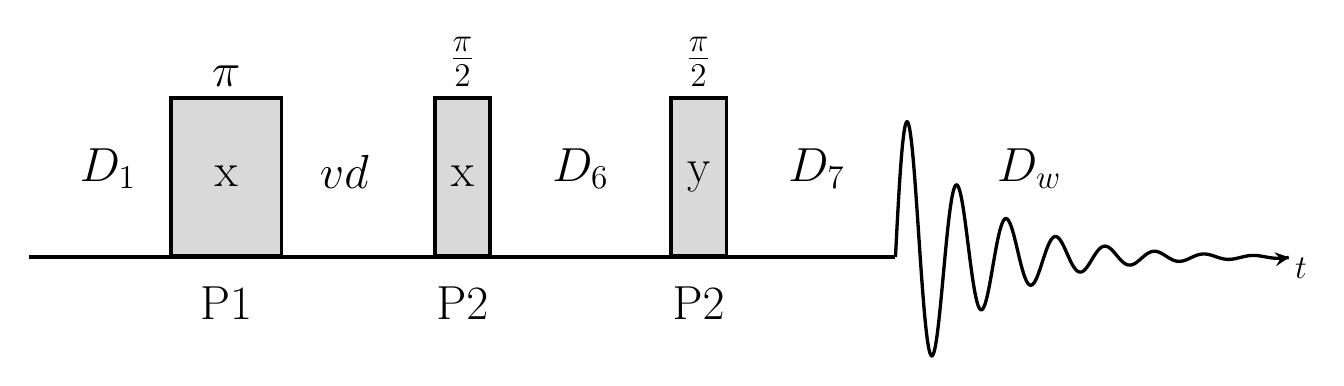
\begin{tikzpicture}[remember picture]
\tikzset{puls/.style={
    rectangle, draw=black, very thick, fill=gray!30 ,minimum width=0.7cm,minimum height=2cm},
    180puls/.style={
    rectangle, draw=black, very thick, fill=gray!30 ,minimum width=1.4cm,minimum height=2cm}
}

    \coordinate (start) at (-3, 0);
    \coordinate (end) at (8, 0);
    \coordinate (rf_180) at ($(-0.5,0)$);
    \coordinate (rf_1) at ($(rf_180) + (3,0)$);
    \coordinate (rf_2) at ($(rf_1) + (3,0)$);
   
    
   
    \coordinate (del_1) at ($(-2,0.5)$);
     \coordinate (vd) at ($(del_1)+(3.0,0)$);
    \coordinate (del_2) at ($(vd) + (3,0)$);
    \coordinate (del_3) at ($(del_2) + (3,0)$);
     \coordinate (signal) at ($(del_3) + (2.7,0)$);  
    
    
      
    \path (rf_180) node[180puls, above, label= \LARGE$\pi$]{\LARGE x};
     \path (rf_180)  node[below,label={[label distance=0 cm]below:{\LARGE P1}} ]{};
    
    \path (rf_1) node[puls, above, label= \LARGE$\frac{\pi}{2}$]{\LARGE x};
     \path (rf_1)  node[below,label={[label distance=0 cm]below:{\LARGE P2}} ]{};
   
   
   
    \path (rf_2) node[puls,above, label= \LARGE$\frac{\pi}{2}$ ]{\LARGE y};
     \path (rf_2)  node[below,label={[label distance=0 cm]below:{\LARGE P2}} ]{};
    
    \draw  (vd) node[above, label= \LARGE $vd$] {};
    \draw  (del_1) node[above, label= \LARGE $D_1$] {};
    \draw  (del_2) node[above, label= \LARGE $D_6$] {};
    \draw  (del_3) node[above, label= \LARGE $D_7$] {};
    \draw  (signal) node[above, label= \LARGE $D_w$] {};

  
     \draw[very thick] ($(start)$ ) -- ( $(end)$ ) node[label={[label distance=-5.5 cm]left:{\large $t$}}, anchor = north] {};
      \def\a{-1}
    \def\b{10}
    \def\c{2}
    \def\N{1000}
    \draw[very thick,samples=\N,variable=\t, domain=0:5,-stealth] (signal) plot({\t+ 8.},  {exp(\a * \t)*\c*sin( \b*\t r)} );

\end{tikzpicture}


\end{document}